
\begin{minipage}{0.38\linewidth}
La figure ci-contre représente un schéma
  de la pyramide de Chéops. C'est une pyramide régulière à base
  carrée, de centre $O$, de côté 227~m et d'arête 217~m.\\
Calcule l'angle $\widehat{OHS}$ (on donnera la valeur approchée
au degré près).
\end{minipage}
\hfill
\begin{minipage}{0.48\linewidth}
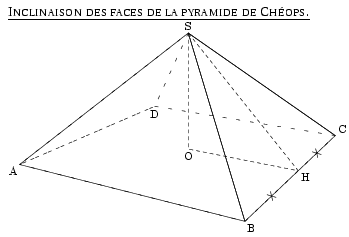
\includegraphics[scale=1]{TR-exo33.png} 
\end{minipage}
\hfill
\begin{minipage}{0.1\linewidth}

\includegraphics[scale=0.7]{qrcodePyramide.png} 
\end{minipage}